\def\problemCode{\LR{Segment Tree}}
\def\problemFarsiTitle{درخت بازه‌ای}

\begin{problem}

با استفاده از 
\LR{fenwick}
تونستیم به پرسش‌های عوض کردن یک خانه و پیدا کردن جمع یک بازه جواب بدیم.
دیدیم که
\LR{fenwick}
برای اینکه جواب پرسش یک بازه رو پیدا کنه، باید پرسش این ویژگی رو داشته باشه که
\LR{partially}
جواب داده بشه. یعنی بتونیم جواب برای بازه
$[l, r]$
رو از روی جواب 
$[1, l - 1]$
و
$[1, r]$
پیدا کنیم. برای مثال این ویژگی رو پرسش‌های 
جمع و ضرب دارند ولی خیلی از عملیات‌ها مثل ماکسیمم و
\LR{gcd}
این ویژگی رو ندارند
.
در ادامه مسئله‌ای که حل می‌کنیم رو توضیح می‌دیم.

آرایه‌ای از اعداد داریم. تعدادی پرسش به یکی از حالات زیر می‌آید:
\begin{itemize}
  \item 
  \LR{change $idx$ $value$}:
    مقدار خانه
    $idx$
    را به
    $value$
    تغییر بده.

  \item 
  \LR{getmax $L$ $R$}:
    ماکسیمم بازه
    $[L, R]$
    را خروجی بده.
\end{itemize}
هدف انجام هر پرسش در 
$\mathcal{O}(\log n)$
می‌باشد که 
$n$
طول آرایه است.

فرض کنید که 
$n = 8$
است.
به درخت زیر توجه کنید.
\usetikzlibrary{trees}

\begin{center}
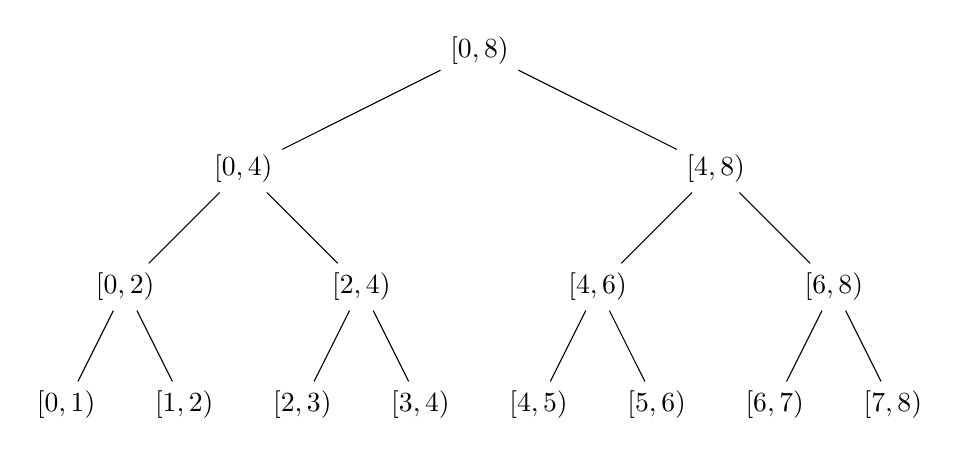
\begin{tikzpicture}[level distance=1.5cm,
  level 1/.style={sibling distance=6cm},
  level 2/.style={sibling distance=3cm},
  level 3/.style={sibling distance=1.5cm}]
  \node{$[0, 8)$}
    child {node {$[0, 4)$}
      child {node {$[0, 2)$}
        child {node {$[0, 1)$}}
        child {node {$[1, 2)$}}
      }
      child {node {$[2, 4)$}
        child {node {$[2, 3)$}}
        child {node {$[3, 4)$}}        
      }
    }
    child {node {$[4, 8)$}
      child {node {$[4, 6)$}
        child {node {$[4, 5)$}}
        child {node {$[5, 6)$}}
      }
      child {node {$[6, 8)$}
        child {node {$[6, 7)$}}
        child {node {$[7, 8)$}}        
      }
    };
\end{tikzpicture}
\end{center}
هر راس این درخت دودویی کامل یک بازه از آرایه را نشان می‌دهد. 
برگ‌های آن بازه‌های تک عضوی هستند و 
بازه هر راس اجتماع بازع دو بچه‌ی آن است. 
تعداد راس‌های این درخت دقیقا
$2n - 1$
است و ارتفاع آن نیز
$\lceil \log_n rceil$
می‌باشد.

در هر راس ماکسیمم بازه مربوط به آن را ذخیره می‌کنیم.
حال بررسی می‌کنیم 
هر تغییر در آرایه چه تغییری در درخت می‌دهد و 
برای جواب دادن به هر پرسش باید چه کنیم.

\mysection{تغییر یک خانه}
ابتدا فرض کنید در مثال 
$n = 8$
مقدار خانه 
$6$
تغییر کند. بدیهی است که راس‌هایی از درخت ممکن است مقدارشان تغییر کند که 
$6$
در بازه‌ی مربوط به آن حضور داشته باشد.
این خانه‌ها در شکل زیر علامت زده شده‌اند.

ویژگی این درخت این است که هر عضو از آرایه در مسیر برگ آن به ریشه حضور دارد.
اگر از ریشه به پایین بیاییم، 
هر اندیسی در بازه مربوط به دقیقا یکی از بچه‌های ریشه وجود دارد.
به طور بازگشتی می‌توان همه راس‌هایی که دچار تغییر می‌شوند را آپدیت کرد.
اگر راس دلخواهی از درخت باید تغییر کند، ابتدا بچه‌ی مربوطه‌اش را تغییر می‌دهیم و سپس مقدار آن را ماکسیمم دو بچه‌اش قرار می‌دهیم.

\usetikzlibrary{trees}

\begin{center}
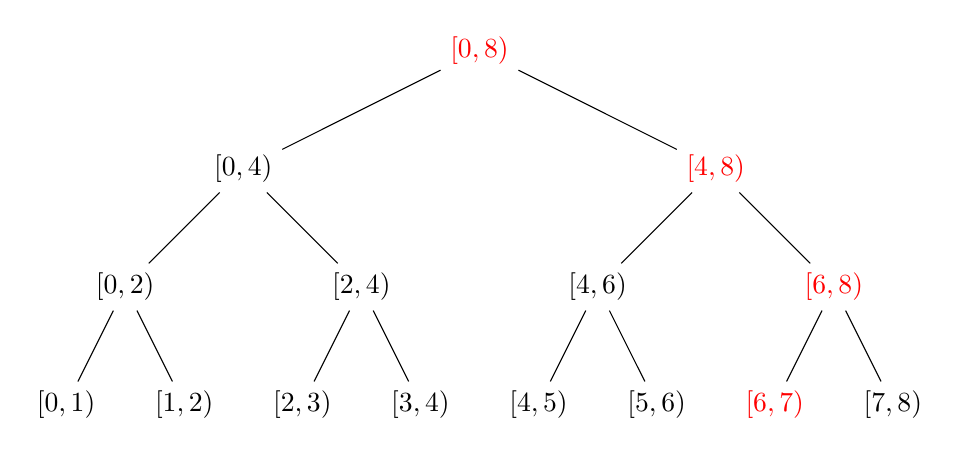
\begin{tikzpicture}[level distance=1.5cm,
  level 1/.style={sibling distance=6cm},
  level 2/.style={sibling distance=3cm},
  level 3/.style={sibling distance=1.5cm}]
  \node{${\color{red}[0, 8)}$}
    child {node {$[0, 4)$}
      child {node {$[0, 2)$}
        child {node {$[0, 1)$}}
        child {node {$[1, 2)$}}
      }
      child {node {$[2, 4)$}
        child {node {$[2, 3)$}}
        child {node {$[3, 4)$}}        
      }
    }
    child {node {${\color{red}[4, 8)}$}
      child {node {$[4, 6)$}
        child {node {$[4, 5)$}}
        child {node {$[5, 6)$}}
      }
      child {node {$\color{red}[6, 8)$}
        child {node {$\color{red}[6, 7)$}}
        child {node {$[7, 8)$}}        
      }
    };
\end{tikzpicture}
\end{center}

شبه‌کد آن به این صورت است.

\LR{
\inputminted{cpp}{codes/segchange.cpp}
}

\mysection{گرفتن یک بازه}
دوباره 
در مثال
$n = 8$
فرض کنید ماکسیمم بازه
$[2, 7)$
را می‌خواهیم پیدا کنیم. از ریشه شروع می‌کنیم و در هر راسی که هستیم به دنبال پیدا کردن
ماکسیمم اشتراک راس و بازه مربوطه هستیم.
اگر بازه درخت کاملا درون بازه پرسش قرار داشت، مقدار ذخیره شده راس درخت را برمی‌گردانیم و 
در غیر این صورت به صورت بازگشتی از دو بچه‌ی آن ماکسیمم اشتراکشان را پیدا می‌کنیم و سپس ماکسیمم دو مقدار بازگردانده شده را برمی‌گردانیم.

\usetikzlibrary{trees}

\begin{center}
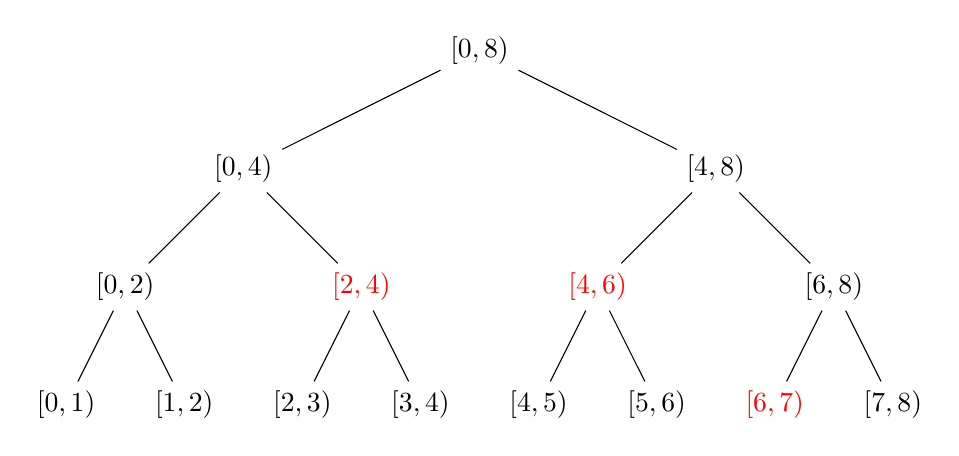
\begin{tikzpicture}[level distance=1.5cm,
  level 1/.style={sibling distance=6cm},
  level 2/.style={sibling distance=3cm},
  level 3/.style={sibling distance=1.5cm}]
  \node{$[0, 8)$}
    child {node {$[0, 4)$}
      child {node {$[0, 2)$}
        child {node {$[0, 1)$}}
        child {node {$[1, 2)$}}
      }
      child {node {$\color{red}[2, 4)$}
        child {node {$[2, 3)$}}
        child {node {$[3, 4)$}}        
      }
    }
    child {node {$[4, 8)$}
      child {node {$\color{red}[4, 6)$}
        child {node {$[4, 5)$}}
        child {node {$[5, 6)$}}
      }
      child {node {$[6, 8)$}
        child {node {$\color{red}[6, 7)$}}
        child {node {$[7, 8)$}}        
      }
    };
\end{tikzpicture}
\end{center}

\LR{
  \inputminted{cpp}{codes/segget.cpp}
}

\mysection{جزئیات پیاده‌سازی}

شماره رئوس درخت مانند شکل زیر است. خاصیت این شماره‌گذاری این است که شماره‌ی بچه‌های راس 
$x$
برابر
$2x$
و
$2x + 1$
می‌باشد.

\usetikzlibrary{trees}

\begin{center}
\begin{tikzpicture}[level distance=1.5cm,
  level 1/.style={sibling distance=6cm},
  level 2/.style={sibling distance=3cm},
  level 3/.style={sibling distance=1.5cm}]
  \node{$1$}
    child {node {$2$}
      child {node {$4$}
        child {node {$8$}}
        child {node {$9$}}
      }
      child {node {$5$}
        child {node {$10$}}
        child {node {$11$}}        
      }
    }
    child {node {$3$}
      child {node {$6$}
        child {node {$12$}}
        child {node {$13$}}
      }
      child {node {$7$}
        child {node {$14$}}
        child {node {$15$}}        
      }
    };
\end{tikzpicture}
\end{center}

\LR{
  \inputminted{cpp}{codes/segcode.cpp}
}

\end{problem}